\section{Specific Requirements}

\subsection{External Interfaces}

\subsection{Functions}

\begin{figure}[H]
  \centering
  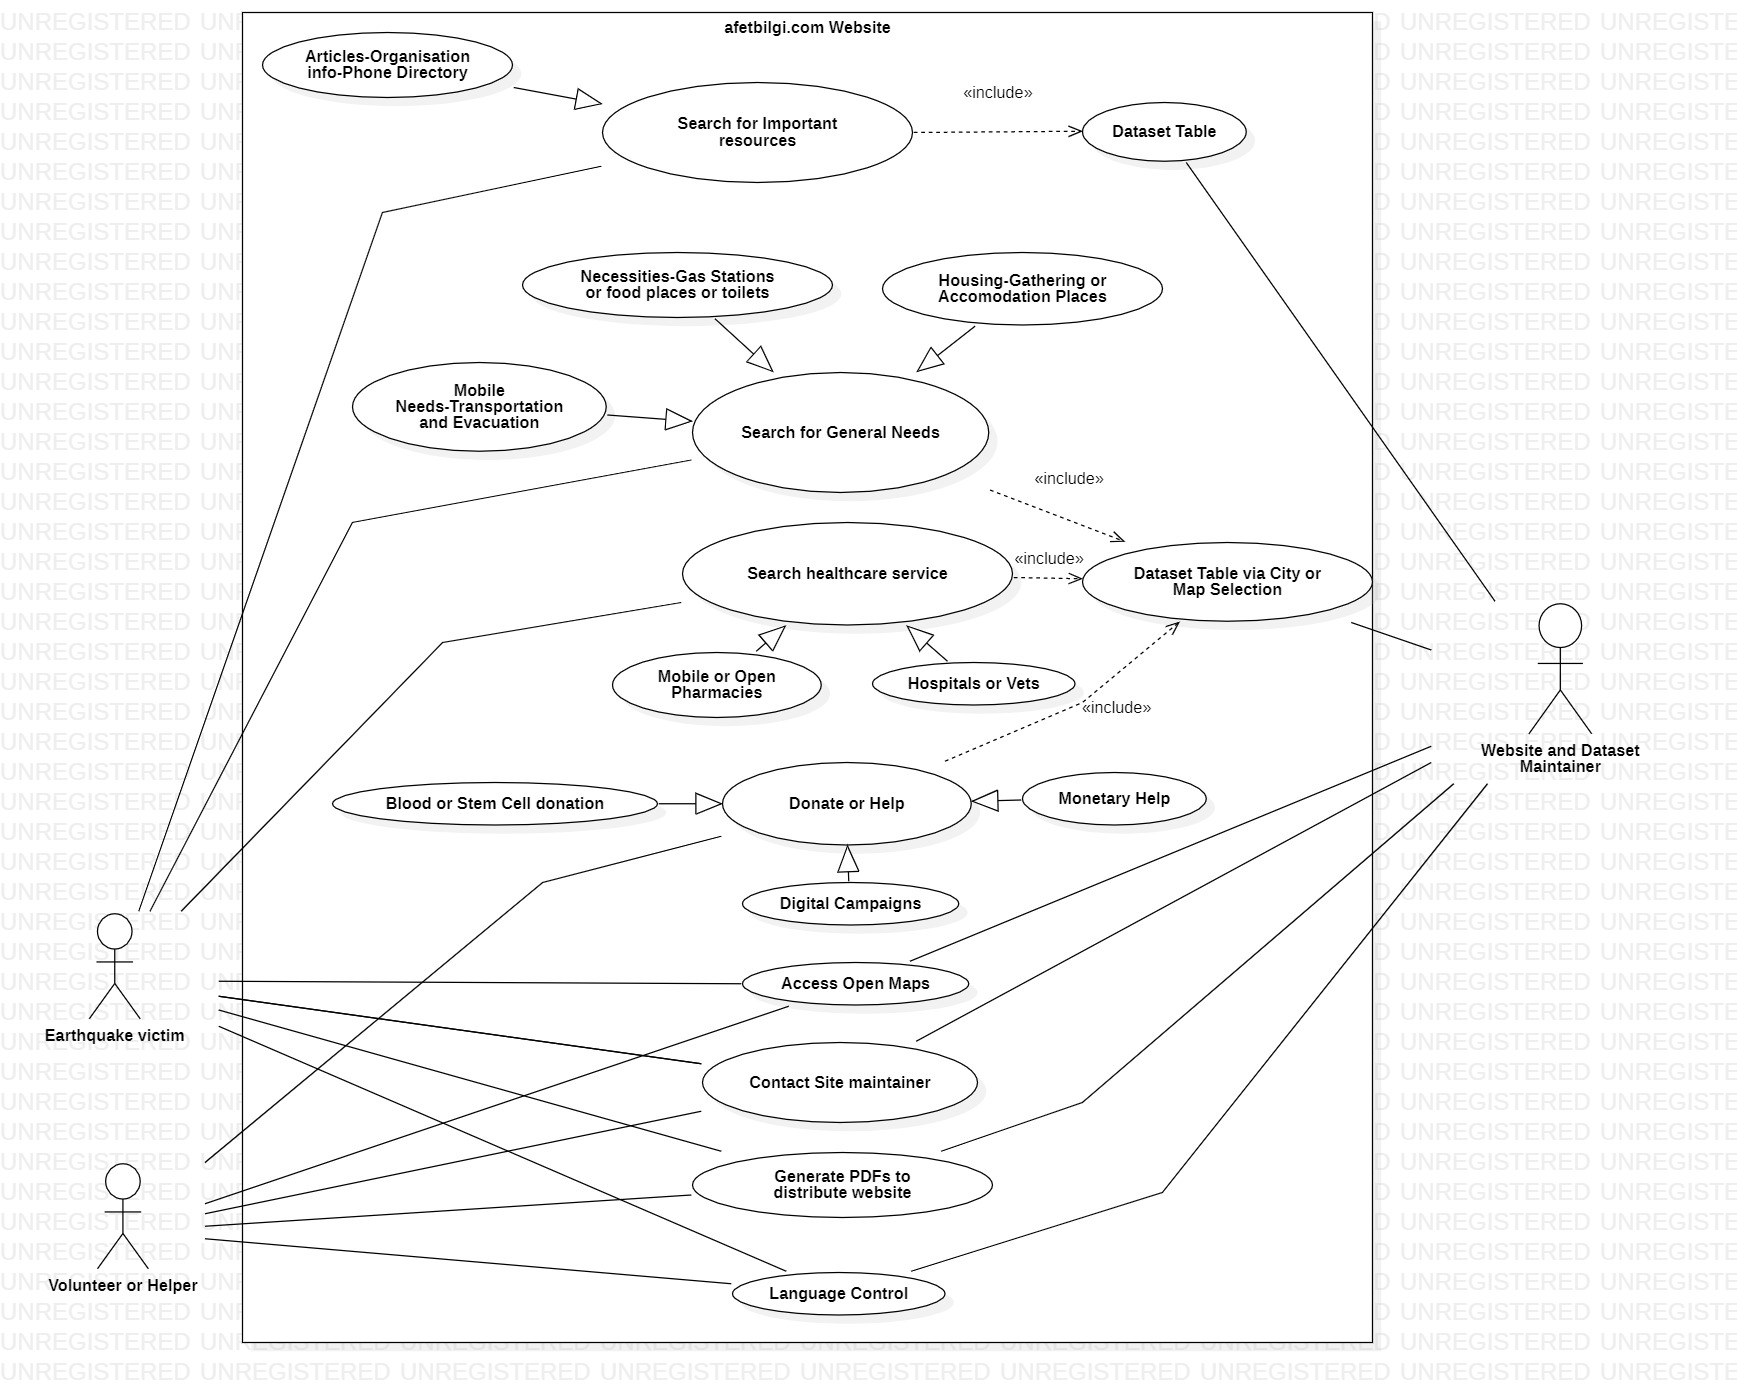
\includegraphics[width=\textwidth]{img/use-case-diagram.jpg}
  \caption{Use Case Diagram for \href{https://afetbilgi.com}{afetbilgi.com}}
\end{figure}

\begin{table}[H]
  \centering
  \begin{tabular}{|p{.3\linewidth}|p{.7\linewidth}|}
    \hline
    \textbf{Use Case ID} & \thetable \\
    \hline
    \textbf{Use-Case Name} & Donate or Help \\
    \hline
    \textbf{Actors} & Volunteer or Helper and Website maintainers \\
    \hline
    \textbf{Description} & Whenever a site user wants to donate or help earthquake victims, he or she can view verified and updated institutions and organisations, which he or she can donate to, on the website to donate to \\
    \hline
    \textbf{Data} & Verified and updated directory of external 3rd party links of welfare and governmental organisations \\
    \hline
    \textbf{Preconditions} & The directory must be updated and verified regularly given the potential monetary usage of the links in the future by the users \\
    \hline
    \textbf{Stimulus} & User clicks on the relevant donation/help methods listed as bold text buttons in the ``\texttt{To Help}'' category on the website \\
    \hline
    \textbf{Basic Flow} & 
        \begin{minipage}[ht]{\linewidth} 
            \begin{enumerate}[label=\textbf{Step \arabic*:},leftmargin=1.5\leftmargin]
                \item User clicks on ``\texttt{Digital solidarity campaigns}''
                \item User selects any of the presented external-3rd party links(presented in a directory)
                \item User redirected to verified 3rd party website
            \end{enumerate}
        \end{minipage} \\
    \hline
    \textbf{Alternative Flow \#1} & 
        \begin{minipage}[ht]{\linewidth} 
            \begin{enumerate}[label=\textbf{Step \arabic*:},leftmargin=1.5\leftmargin]
                \item User clicks on ``\texttt{Other donation}''
                \item User selects relevant city
                \item User selects verified helper links of individuals/smaller organisations along with their contact details
                \item User clicks on any link and escorted out to a 3rd party site
            \end{enumerate}
        \end{minipage} \\
    \hline
    \textbf{Alternative Flow \#2} &
    \begin{minipage}[ht]{\linewidth} 
            \begin{enumerate}[label=\textbf{Step \arabic*:},leftmargin=1.5\leftmargin]
                \item User clicks on ``\texttt{Kizilay Blood Donation Places}''
                \item User automatically redirected to primary verified 3rd party site of governmental organisation accepting blood donations
            \end{enumerate}
        \end{minipage} \\
    \hline
    \textbf{Exception Flow} & - \\
    \hline
    \textbf{Post Conditions} & User is redirected to a verified external website out of the afetbilgi.com domain \\
    \hline
  \end{tabular}
  \caption{Use Case - Donate or Help}
\end{table}

\begin{table}[H]
  \centering
  \begin{tabular}{|p{.3\linewidth}|p{.7\linewidth}|}
    \hline
    \textbf{Use Case ID} & \thetable \\
    \hline
    \textbf{Use-Case Name} & Access open maps \\
    \hline
    \textbf{Actors} & Volunteers or Victims, Website maintainers \\
    \hline
    \textbf{Description} & Users can view current location with respect to places in need of help and use interactive map view to track down relevant places offering help (verified by site maintainers) via GPS location \\
    \hline
    \textbf{Data} & Interactive Map View with relevant place descriptions to navigate on \\
    \hline
    \textbf{Preconditions} & Places ought to be verified, properly categorised and color coded for easy understanding by site user \\
    \hline
    \textbf{Stimulus} & User drags mouse around on map view involving GPS after clicking on the map button anywhere on screen or calling \href{https://maps.afetbilgi.com}{\texttt{maps.afetbilgi.com}} directly in the browser \\
    \hline
    \textbf{Basic Flow} & 
        \begin{minipage}[ht]{\linewidth} 
            \begin{enumerate}[label=\textbf{Step \arabic*:},leftmargin=1.5\leftmargin]
                \item User is shown his current location with respect to to rest of Turkey
                \item Users can zoom in or out of Turkey's map and track themselves to needy areas as per color codes and categorisation
                \item User can click on a tracked down helping house, restaurant, etc. and be greeted by a pop up box with description and relevant links to third party sites or Google Maps routes
                \item User can click on the links and escorted out to 3rd party websites or Google Maps website
            \end{enumerate}
        \end{minipage} \\
    \hline
    \textbf{Alternative Flow \#1} & 
    \begin{minipage}[ht]{\linewidth} 
            \begin{enumerate}[label=\textbf{Step \arabic*:},leftmargin=1.5\leftmargin]
                \item User can select zoom in or out along with clicking on the camera icon
                \item User can save map screenshot for later use or distribution
            \end{enumerate}
        \end{minipage} \\
    \hline
    \textbf{Alternative Flow \#2} & - \\
    \hline
    \textbf{Exception Flow} & - \\
    \hline
    \textbf{Post Conditions} & User ends up on verified external website outside of \href{https://afetbilgi.com}{\texttt{afetbilgi.com}} domain \\
    \hline
  \end{tabular}
  \caption{Use Case - Access open maps}
\end{table}

\begin{table}[H]
  \centering
  \begin{tabular}{|p{.3\linewidth}|p{.7\linewidth}|}
    \hline
    \textbf{Use Case ID} & \thetable \\
    \hline
    \textbf{Use-Case Name} & Generate PDFs to distribute website \\
    \hline
    \textbf{Actors} & Volunteers or victims \\
    \hline
    \textbf{Description} & Users can save filtered out website directories for later use given possible lack of electrical or network necessities in these earthquake stricken areas\\
    \hline
    \textbf{Data} & Separate downloadable PDF documents after selecting relevant cities \\
    \hline
    \textbf{Preconditions} & User is able to select entire cities with verified directory links and contact information  \\
    \hline
    \textbf{Stimulus} & User clicks on PDF icon button anywhere on the website \\
    \hline
    \textbf{Basic Flow} &
        \begin{minipage}[ht]{\linewidth} 
            \begin{enumerate}[label=\textbf{Step \arabic*:},leftmargin=1.5\leftmargin]
                \item User clicks on PDF icon anywhere on website
                \item User selects city
                \item Document is loaded and enabled for download by the user with the relevant city and categories highlighted on it
            \end{enumerate}
        \end{minipage} \\
    \hline
    \textbf{Alternative Flow \#1} & - \\
    \hline
    \textbf{Alternative Flow \#2} & - \\
    \hline
    \textbf{Exception Flow} & - \\
    \hline
    \textbf{Post Conditions} & Site user has received well formatted and legible generated PDF document with relevant hyperlinks and contact details of verified directories  \\
    \hline
  \end{tabular}
  \caption{Use Case - Generate PDFs to distribute website}
\end{table}

\subsection{Usability Requirements}

\subsection{Performance Requirements}

\subsection{Logical Database Requirements}

\subsection{Design Constraints}

\subsection{System Attributes}

\subsection{Supporting Information}
